\documentclass[a4paper, 12pt]{article}
%%% Работа с русским языком
\usepackage{cmap}					% поиск в PDF
\usepackage{mathtext} 				% русские буквы в фомулах
\usepackage{amsmath}
\usepackage[T2A]{fontenc}			% кодировка
\usepackage[utf8]{inputenc}			% кодировка исходного текста
\usepackage[english,russian]{babel}	% локализация и переносы
\usepackage{hyperref}               % ссылки
\usepackage{graphicx}               
\usepackage{amsmath}



\author{Пермяков Андрей А-13б-19}
\title{ДЗ1. Регулярные языки и конечные автоматы}
\date{}

\begin{document}

\maketitle

% 1
\section{Построить конечный автомат, распознающий язык}
Ответом на данное задание является конечный автомат, распознающий описанный язык. Автомат должен быть детерминированным.


$$ 1. L = \{w \in \{a,b,c\}^* | |w|_c = 1 \} $$

\begin{center}
    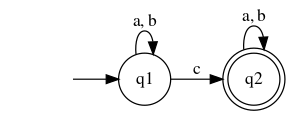
\includegraphics[scale=0.7]{graph1_1.png}
\end{center}

$$2. L = \{w \in \{a,b\}^* | |w|_a \leq 2, |w|_b \geq 2 \}$$

\begin{center}
    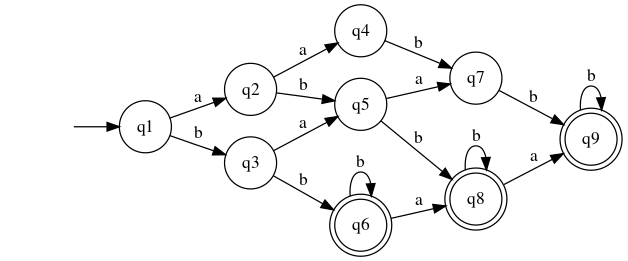
\includegraphics[scale=0.7]{graph1_2.png}
\end{center}
$$3. L = \{w \in \{a,b\}^* | |w|_a \neq |w|_b \}$$
Для такого языка невозможно построить КА, так как необходимо считывать количество символов a и b. Поэтому построим для языка, в котором символы чередуются.
\begin{center}
    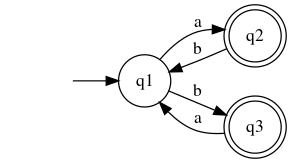
\includegraphics[scale=0.7]{graph1_3.png}
\end{center}
$$4. L = \{w \in \{a,b\}^* | ww = www \}$$
\begin{center}
    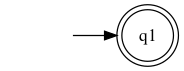
\includegraphics[scale=0.7]{graph1_4.png}
\end{center}


% 2
\section{Построить конечный автомат, используя прямое произведение}
Ответом на данное задание является конечный автомат, распознающий описанный язык. Требуется, чтобы он был построен при помощи прямого произведения ДКА и его свойств.

$$1. L_1 = \{ w \in \{a,b\}^* | |w|_a \geq 2 \land |w|_b \geq 2\}$$

$$2. L_2 = \{ w \in \{a,b\}^* | |w| \geq 3 \land |w| \text{ нечетное} \}$$
$$3. L_3 = \{ w \in \{a,b\}^* | |w|_a \text{ четно} \land |w|_b \text{ кратно трем} \}$$
$$4. L_4 = \overline{L_3}$$
$$5. L_5 = L_2 \backslash L_3$$

% 3
\section{Построить минимальный ДКА по регулярному выражению}
Ответом на данное задание является минимальный ДКА, который допускает тот же язык, что описывается регулярным выражением.

$$1. (ab + aba)^*$$
$$2. a(a(ab)^*b)^*(ab)^*$$
$$3. (a + (a + b)(a + b)b)^*$$
$$4. (b + c)((ab)^*c + (ba)^*)^*$$
$$5. (a + b)^+(aa + bb + abab + baba)(a + b)^+$$


% 4
\section{Определить является ли язык регулярным или нет}
Ответом на данное задание является конечный автомат, если язык регулярен, либо доказательство нерегулярности языка при помощи леммы о разрастании.
$$1. L = \{(aab)^nb(aba)^m | n \geq 0, m \geq 0\}$$
$$1. L = \{uaav | u \in \{a,b\}^*, v \in \{a,b\}^*, |u|_b \geq |v|_a\}$$
$$1. L = \{a^mw | w \in \{a, b\}^*, 1 \leq |w|_b \leq m  \}$$
$$1. L = \{ a^kb^ma^n | k = n \lor m > 0\}$$
$$1. L = \{ ucv | u \in \{a,b\}^*, v \in \{a,b\}^*, u \neq v^R \}$$

% 5
\section{Реализовать алгоритмы}
Ответом на данное задание является работающая программа на выбранном языке программирования, покрытая юнит-тестами.

В рамках своего выполнения программа должна генерировать текстовый документ с картинками, показывающий процесс построения автомата (к примеру, Markdown с графиками на Graphviz).\\
1. Построение ДКА по НКА с $\lambda$-переходами \\
2. Прямое произведение языков, с возможностью построить пересечение, объединение и разность.

\end{document}
